\section{Subgrupos, Generadores, Retículos y Grupos cíclicos}

\begin{ejercicio}\label{ej:3.1}
    Describir todos los elementos de los grupos alternados $A_n$, consistentes en las permutaciones pares del $S_n$ correspondiente, para:
    \begin{enumerate}
        \item $n = 2$.
        \begin{align*}
            S_2 &= \{1, (1\ 2)\}\\
            A_2 &= \{1\}
        \end{align*}
        \item $n = 3$.
        \begin{align*}
            S_3 &= \{1, (1\ 2), (1\ 3), (2\ 3), (1\ 2\ 3), (1\ 3\ 2)\}\\
            A_3 &= \{1, (1\ 2\ 3), (1\ 3\ 2)\}
        \end{align*}
        \item $n = 4$.
        \begin{align*}
            S_4 &= \{1, (1\ 2), (1\ 3), (1\ 4), (2\ 3), (2\ 4), (3\ 4), (1\ 2\ 3), (1\ 2\ 4), (1\ 3\ 2), (1\ 3\ 4),\\&\hspace{2cm} (1\ 4\ 2), (1\ 4\ 3), (2\ 3\ 4), (2\ 4\ 3), (1\ 2\ 3\ 4), (1\ 2\ 4\ 3), (1\ 3\ 2\ 4),\\&\hspace{2cm} (1\ 3\ 4\ 2), (1\ 4\ 2\ 3), (1\ 4\ 3\ 2), (1\ 2)(3\ 4), (1\ 3)(2\ 4), (1\ 4)(2\ 3)\}\\
            A_4 &= \{1, (1\ 2\ 3), (1\ 2\ 4), (1\ 3\ 2), (1\ 3\ 4), (1\ 4\ 2), (1\ 4\ 3), (2\ 3\ 4), (2\ 4\ 3),\\&\hspace{2cm} (1\ 2)(3\ 4), (1\ 3)(2\ 4), (1\ 4)(2\ 3)\}
        \end{align*}
    \end{enumerate}
\end{ejercicio}

\begin{ejercicio}\label{ej:3.2}
    Sea $D_n$ el grupo diédrico. Demostrar que el subgrupo de $D_n$ generado por los elementos $\{r^js, r^ks\}$ es todo el grupo $D_n$ siempre que $0 \leq j < k < n$ y $\mcd(k - j, n) = 1$.\\

    Haciendo uso de que $D_n = \langle r,s\rangle$, veamos que:
    \begin{align*}
        \langle r^js, r^ks\rangle &= D_n
    \end{align*}
    \begin{description}
        \item[$\subseteq)$] Como $r,s\in D_n$, entonces $r^js, r^ks\in D_n$. Por ser $D_n$ un grupo, en particular es cerrado para el producto y para inversos, por lo que $\langle r^js, r^ks\rangle\subseteq D_n$.
        
        \item[$\supseteq)$] Veamos en primer lugar que $r\in\langle r^js, r^ks\rangle$. Sabemos que:
        \begin{equation*}
            (r^js)^{-1} = sr^{-j}\in \langle r^js, r^ks\rangle
        \end{equation*}

        Por tanto, como $r^ks\in\langle r^js, r^ks\rangle$, entonces:
        \begin{equation*}
            r^ks(r^js)^{-1} = r^kssr^{-j} = r^{k-j}\in\langle r^js, r^ks\rangle
        \end{equation*}

        Como $\mcd(k-j,n)=1$, entonces existe $m\in\bb{Z}$, con $0\leq m<n$, tal que $m(k-j)=qn+1$ para algún $q\in\bb{Z}$. Por tanto:
        \begin{equation*}
            (r^{k-j})^m = r^{m(k-j)} = r^{qn+1} = r\in\langle r^js, r^ks\rangle
        \end{equation*}

        Por último, veamos que $s\in\langle r^js, r^ks\rangle$. Como $r\in\langle r^js, r^ks\rangle$, entonces:
        \begin{equation*}
            r^{n-j}r^js = r^{n-j+j}s = s\in\langle r^js, r^ks\rangle
        \end{equation*}

        Por tanto, $r,s\in\langle r^js, r^ks\rangle$, y por ser $D_n = \langle r,s\rangle$, entonces $D_n\subset \langle r^js, r^ks\rangle$.
    \end{description}
\end{ejercicio}

\begin{ejercicio}\label{ej:3.3}~
    \begin{enumerate}
        \item Demostrar que el subgrupo de $\SL_2(\bb{Z}_3)$ generado por los elementos
        \[
            i = \begin{pmatrix}
                0 & -1 \\
                1 & 0
            \end{pmatrix}, \quad j = \begin{pmatrix}
                1 & 1 \\
                1 & -1
            \end{pmatrix}
        \]
        es isomorfo al grupo cuaternio $Q_2$.\\

        Por la propiedad transitiva de la isomorfia, basta con encontrar un isomorfismo entre $\SL_2(\bb{Z}_3)$ y:
        \begin{equation*}
            Q_2^{abs} = \langle x,y\mid x^4=1,\ y^2=x^2,\ yx=x^{-1}y\rangle
        \end{equation*}

        Comprobamos que $i,j$ cumplen las relaciones de $Q_2^{abs}$:
        \begin{align*}
            i^2 &= \begin{pmatrix}
                -1 & 0 \\
                0 & -1
            \end{pmatrix}\\
            j^2 &= \begin{pmatrix}
                2 & 0 \\
                0 & 2
            \end{pmatrix} = \begin{pmatrix}
                -1 & 0 \\
                0 & -1
            \end{pmatrix}\\
            ji &= \begin{pmatrix}
                1 & -1 \\
                -1 & -1
            \end{pmatrix}\\
            i^3j &= \begin{pmatrix}
                1 & -1 \\
                -1 & -1
            \end{pmatrix}
        \end{align*}

        Por tanto, $i,j$ cumplen las relaciones de $Q_2^{abs}$. Por el Teorema de Dyck, existe un único homomorfismo $f:Q_2^{abs}\to\langle i,j\rangle$ tal que $f(x)=i$ y $f(y)=j$.
        \begin{itemize}
            \item Como $i,j\in\langle i,j\rangle$ son un generador de $\langle i,j\rangle$, entonces se trata de un epimorfismo.
            \item Para terminar de ver que es un isomorfismo, basta con comprobar que $|Q_2^{abs}|=|\langle i,j\rangle|$. Sabemos que:
            \begin{align*}
                \langle i,j\rangle &= \{1,i,i^2,i^3,j,ij,i^2j,i^3j\}\\
                |Q_2^{abs}| &= 8 = |\langle i,j\rangle|
            \end{align*}

            Por tanto, $f$ es un isomorfismo.
        \end{itemize}
        Por tanto, $\langle i,j\rangle\cong Q_2^{abs}\cong Q_2$.
        \item Demostrar que $\SL_2(\bb{Z}_3)$ y $S_4$ son dos grupos de orden 24 que no son isomorfos.
        \begin{observacion}
            Demostrar que $S_4$ no puede contener a ningún subgrupo isomorfo a $Q_2$.
        \end{observacion}
        
        Tenemos que:
        \begin{equation*}
            Q_2 = \{\pm 1, \pm i, \pm j, \pm k\}
        \end{equation*}

        Los órdenes de los elementos de $Q_2$ son:
        \begin{equation*}
            O(\pm i)= O(\pm j)= O(\pm k)=4\qquad O(-1)=2
        \end{equation*}

        Supongamos ahora $\exists H\leq S_4$ tal que $H\cong Q_2$. Por lo pronto, sabemos que $1\in H$ y $|H|=8$.
        Además, como los isomorfismos mantienen los órdenes, sabemos que en $H$ habrá $6$ elementos distintos de orden 4 y $1$ de orden 2. Como en $S_4$ tan solo hay $6$ elementos de orden 4, entonces $H$ ha de contener a todos los elementos de orden 4 de $S_4$; es decir:
        \begin{equation*}
            \{1, (1\ 2\ 3\ 4), (1\ 2\ 4\ 3), (1\ 3\ 2\ 4), (1\ 3\ 4\ 2), (1\ 4\ 2\ 3), (1\ 4\ 3\ 2)\}\subseteq H
        \end{equation*}

        Por tanto, ya tenemos $7$ elementos de $H$, y sabemos que el restante es de orden $2$ (no sabemos si es una transposición o un producto de dos transposición disjuntas). Por ser $H$ un grupo, tenemos que es cerrado para productos, por lo que:
        \begin{equation*}
            (1\ 2\ 3\ 4)(1\ 2\ 4\ 3)=(1\ 3\ 2)\in H
        \end{equation*}
        No obstante, hemos encontrado un elemento de orden $3$ perteneciente a $H$, lo cual es una contradicción. Por tanto, no puede existir un subgrupo de $S_4$ isomorfo a $Q_2$.\\

        Para demostrar lo pedido, supongamos que $\exists f:\SL_2(\bb{Z}_3)\to S_4$ un isomorfismo, y consideramos la restricción a $Q=\langle i,j\rangle\cong Q_2$. Sabemos que la siguiente aplicación es un isomorfismo:
        \Func{f_{\big| Q}}{Q}{f_{\ast}(Q)}{x}{f(M)}

        Por tanto, $Q_2\cong Q\cong f_{\ast}(Q)$. Además, como $f_\ast$ es un homomorfismo y se tiene $Q< \SL_2(\bb{Z}_3)$, entonces $f_{\ast}(Q)< S_4$. Por tanto, hemos encontrado un subgrupo de $S_4$ isomorfo a $Q_2$, lo cual es una contradicción por lo que hemos demostrado anteriormente. Por tanto, $\SL_2(\bb{Z}_3)\ncong S_4$.
    \end{enumerate}
\end{ejercicio}

\begin{ejercicio}\label{ej:3.4}
    Razonar que un subconjunto no vacío $X \subseteq G$ de un grupo $G$ es un subgrupo de $G$ si, y sólo si, $X = \langle X \rangle$.
    \begin{description}
        \item[$\Longrightarrow)$] Supongamos que $X$ es un subgrupo de $G$, y veamos que $X = \langle X \rangle$. \begin{description}
            \item[$\subseteq)$] Por definición de subgrupo generado por un conjunto, $X\subseteq\langle X\rangle$.
            \item[$\supseteq)$] Veamos que $\langle X\rangle\subseteq X$. Dado $x\in \langle X\rangle$, entonces $x$ es una combinación de elementos de $X$ mediante el producto y el inverso. Por ser $X$ un subgrupo, en particular es un grupo, por lo que es cerrado para el producto y para inversos. Por tanto, $x\in X$.
        \end{description}

        Por tanto, $X = \langle X\rangle$.
        \item[$\Longleftarrow)$] Supongamos que $X = \langle X\rangle$, y veamos que $X$ es un subgrupo de $G$. Por definición, $\langle X\rangle$ es el menor subgrupo de $G$ que contiene a $X$. Por tanto, $X$ es un subgrupo de $G$.
    \end{description}
\end{ejercicio}

\begin{ejercicio}\label{ej:3.5}
    Sean $a, b \in G$ dos elementos de un grupo que conmutan entre sí, esto es, para los que $ab = ba$, y de manera que sus órdenes son primos relativos, esto es, $\mcd(O(a), O(b)) = 1$.
    \begin{enumerate}
        \item Razonar que $\langle a \rangle \cap \langle b \rangle = \{1\}$.
        
        \begin{description}
            \item[Opicón 1]
            
            Puesto que la intersección de dos subgrupos es un subgrupo, sabemos que $\langle a\rangle\cap\langle b\rangle$ es un subgrupo de $G$, y por tanto $1\in \langle a\rangle\cap\langle b\rangle\neq \emptyset$. Por tanto, podemos considerar $x\in \langle a\rangle\cap\langle b\rangle$.

            Como menciona el $\mcd(O(a),O(b))$, podemos considerar que ambos órdenes son finitos. Por el Teorema de Lagrange, sabemos que:
            \begin{align*}
                |\langle a\rangle\cap \langle b\rangle|&\mid |\langle a\rangle|=O(a)\\
                |\langle a\rangle\cap \langle b\rangle|&\mid |\langle b\rangle|=O(b)
            \end{align*}

            Por tanto, $|\langle a\rangle\cap \langle b\rangle|$ es divisor común de $O(a)$ y $O(b)$, y por ser $\mcd(O(a),O(b))=~1$, entonces $|\langle a\rangle\cap \langle b\rangle|=1$. Por tanto, $\langle a\rangle\cap \langle b\rangle=\{1\}$.

            \item[Opción 2]
            
            Demostrémoslo por doble inclusión.
            \begin{description}
                \item[$\supseteq)$] Como $\langle a\rangle$ y $\langle b\rangle$ son subgrupos de $G$, entonces $\langle a\rangle\cap \langle b\rangle$ es un subgrupo de $G$, y en particular es un grupo. Por tanto, $1\in \langle a\rangle\cap \langle b\rangle$.
                
                \item[$\subseteq)$] Sea $x\in \langle a\rangle\cap \langle b\rangle$.
                \begin{itemize}
                    \item Como $x\in \langle a\rangle$, entonces $x=a^s$ para algún $s\in\bb{Z}$.
                    \item Como $x\in \langle b\rangle$, entonces $x=b^t$ para algún $t\in\bb{Z}$.
                \end{itemize}

                Por tanto:
                \begin{equation*}
                    1=(a^{O(a)})^s = (a^s)^{O(a)} = x^{O(a)} = (b^t)^{O(a)} = b^{tO(a)}\implies O(b)\mid tO(a)
                \end{equation*}

                Como $\mcd(O(a),O(b))=1$, entonces $O(b)\mid t$, por lo que $\exists k\in\bb{Z}$ tal que $t=kO(b)$. Por tanto:
                \begin{equation*}
                    x=b^t=b^{kO(b)}=(b^{O(b)})^k=1^k=1
                \end{equation*}

                Por tanto, $\langle a\rangle\cap \langle b\rangle\subset \{1\}$.
            \end{description}
        \end{description}

        \item Demostrar que $O(ab) = O(a)O(b)$.
        
        Puesto que conmutan, tenemos que:
        \begin{equation*}
            (ab)^k=a^kb^k\qquad \forall k\in\bb{Z}
        \end{equation*}

        Por comodidad, sean $O(a)=n$ y $O(b)=m$.
        \begin{equation*}
            (ab)^{nm}=a^{nm}b^{nm}=(a^n)^m(b^m)^n=1
        \end{equation*}

        Supongamos ahora $t\in \bb{N}$ tal que $(ab)^t=1$. 
        \begin{equation*}
            \hspace{-1cm}1=(ab)^t=a^tb^t\implies a^t=b^{-t}\in \langle a\rangle\cap \langle b\rangle=\{1\}\implies \left\{\begin{array}{c}
                a^t=1\Longrightarrow n\mid t\\
                a^t=1\Longrightarrow m\mid t
            \end{array}\right\}\stackrel{(\ast)}{\Longrightarrow} nm\mid t
        \end{equation*}
        donde en $(\ast)$ hemos usado que $\mcd(n,m)=1$. Por tanto:
        \begin{equation*}
            O(ab)=nm=O(a)O(b)
        \end{equation*}
    \end{enumerate}
\end{ejercicio}

\begin{ejercicio}\label{ej:3.6}
    Encontrar un grupo $G$ y elementos $a, b \in G$ tales que sus órdenes sean primos relativos, pero para los que no se verifique la igualdad $O(ab) = O(a)O(b)$ del ejercicio anterior.\\

    En primer lugar, hemos de tener que no conmuten. Por tanto, consideremos el grupo $S_3$ y los elementos:
    \begin{align*}
        a &= (1\ 2)\\
        b &= (1\ 2\ 3)
    \end{align*}

    Tenemos que $O(a)=2$ y $O(b)=3$, y por tanto $\mcd(O(a),O(b))=1$. Además, $O(a)O(b)=6$. Supongamos que $\exists \sigma\in S_3$ tal que $O(\sigma)=6$. Por tanto, el mínimo común múltiplo de los ciclos disjuntos que la descomponen debe ser 6. Sin embargo, esto no es posible, porque en $S_3$ tan solo hay elementos de orden 1, 2 y 3. Por tanto, $O(ab)\neq O(a)O(b)$.
\end{ejercicio}

\begin{ejercicio}\label{ej:3.7}
    Sea $G$ un grupo y $a, b \in G$ dos elementos de orden finito. ¿Es $ab$ necesariamente de orden finito?
    \begin{observacion}
        Considerar el grupo $\GL_2(\bb{Q})$ y los elementos
        \[
            a = \begin{pmatrix}
                0 & -1 \\
                1 & 0
            \end{pmatrix}, \quad b = \begin{pmatrix}
                0 & 1 \\
                -1 & 1
            \end{pmatrix}.
        \]
    \end{observacion}
    Calculemos el orden de $a$ y $b$:
    \begin{align*}
        a^2&=\begin{pmatrix}
            -1 & 0 \\
            0 & -1
        \end{pmatrix}=-I_2\implies O(a)=4\\
        b^2&=\begin{pmatrix}
            -1 & 1 \\
            -1 & 0
        \end{pmatrix}\\
        b^3&=\begin{pmatrix}
            -1 & 0 \\
            0 & -1
        \end{pmatrix}=-I_2\implies O(b)=6
    \end{align*}

    Calculamos ahora el orden de $ab$. Por inducción, demostraremos que:
    \begin{equation*}
        (ab)^n=\begin{pmatrix}
            1 & -n \\
            0 & 1
        \end{pmatrix}
    \end{equation*}
    \begin{itemize}
        \item \ul{Caso base:} $n=1$.
        \begin{equation*}
            (ab)^1=\begin{pmatrix}
                0 & -1 \\
                1 & 0
            \end{pmatrix}\begin{pmatrix}
                0 & 1 \\
                -1 & 1
            \end{pmatrix}=\begin{pmatrix}
                1 & -1 \\
                0 & 1
            \end{pmatrix}
        \end{equation*}

        \item \ul{Supuesto cierto para $n$, demostramos para $n+1$:}
        \begin{align*}
            (ab)^{n+1}&=(ab)^n(ab)=\begin{pmatrix}
                1 & -n \\
                0 & 1
            \end{pmatrix}\begin{pmatrix}
                1 & -1 \\
                0 & 1
            \end{pmatrix}
            =\begin{pmatrix}
                1 & -(n+1) \\
                0 & 1
            \end{pmatrix}
        \end{align*}
    \end{itemize}

    Por tanto, como en $(ab)^n\neq I_2$ para todo $n\in\bb{N}$, entonces $O(ab)=\infty$.
\end{ejercicio}

\begin{ejercicio}\label{ej:3.8}
    En el grupo $S_3$ se considera el conjunto
    \[
        H = \{1, (1\ 2\ 3), (1\ 3\ 2)\}.
    \]
    \begin{enumerate}
        \item Demostrar que $H$ es un subgrupo de $S_3$.
        
        \begin{description}
            \item[Opción 1.]
            
            Por ser $S_3$ finito, tan solo hemos de comprobar que $H$ es cerrado para el producto. Como vimos, no es necesario comprobar si uno de los elementos es el neutro.
            \begin{align*}
                (1\ 2\ 3)^2&=(1\ 3\ 2)\\
                (1\ 3\ 2)^2&=(1\ 2\ 3)\\
                (1\ 2\ 3)(1\ 3\ 2)&=1\\
                (1\ 3\ 2)(1\ 2\ 3)&=1
            \end{align*}

            Por tanto, $H< S_3$.

            \item[Opción 2.] Demostremos que $H=\langle (1\ 2\ 3)\rangle$.
            \begin{description}
                \item[$\subseteq)$] Tan solo será necesario ver que $(1\ 2\ 3)^2=(1\ 3\ 2)$, y se tendría de manera inmediata que $H\subseteq\langle (1\ 2\ 3)\rangle$.
                
                \item[$\supseteq)$] Sea $x\in\langle (1\ 2\ 3)\rangle$. Entonces $x=(1\ 2\ 3)^n$ para algún $n\in\bb{Z}$. Como $O((1\ 2\ 3))=3$, entonces $n\in\{0,1,2\}$. Por tanto:
                \begin{equation*}
                    x\in  \{(1\ 2\ 3)^0, (1\ 2\ 3)^1, (1\ 2\ 3)^2\} = \{1, (1\ 2\ 3), (1\ 3\ 2)\} = H
                \end{equation*}
            \end{description}
        \end{description}
        \item Describir las diferentes clases de $S_3$ módulo $H$.
        
        Por el Teorema de Lagrange, sabemos que:
        \begin{equation*}
            |S_3|=[S_3:H]\cdot |H|\Longrightarrow [S_3:H]=\dfrac{6}{3}=2\Longrightarrow |S_3/\prescript{}{H}{\sim}| = |S_3/\sim_H|=2
        \end{equation*}

        Calculamos ahora las clases de equivalencia de $S_3/\prescript{}{H}{\sim}$:
        \begin{align*}
            1H &= \{1x\mid x\in H\} = \{1, (1\ 2\ 3), (1\ 3\ 2)\} = H\\
            (1\ 2)H &= \{(1\ 2)x\mid x\in H\} = \{(1\ 2), (1\ 2)(1\ 2\ 3), (1\ 2)(1\ 3\ 2)\} = \{(1\ 2), (2\ 3), (1\ 3)\}\neq H
        \end{align*}
        Como ya hemos encontrado dos clases de equivalencia distintas, entonces hemos encontrado todas las posibles.
        \begin{equation*}
            S_3/\prescript{}{H}{\sim} = \{H, (1\ 2)H\}
        \end{equation*}

        Calculamos ahora las clases de equivalencia de $S_3/\sim_H$:
        \begin{align*}
            H1 &= \{x1\mid x\in H\} = \{1, (1\ 2\ 3), (1\ 3\ 2)\} = H\\
            H(1\ 2) &= \{x(1\ 2)\mid x\in H\} = \{(1\ 2), (1\ 2\ 3)(1\ 2), (1\ 3\ 2)(1\ 2)\} = \{(1\ 2), (1\ 3), (2\ 3)\}\neq H
        \end{align*}

        Por tanto, hemos encontrado todas las clases de equivalencia de $S_3/\sim_H$.
        \begin{equation*}
            S_3/\sim_H = \{H, H(1\ 2)\}
        \end{equation*}
    \end{enumerate}
\end{ejercicio}

\begin{ejercicio}\label{ej:3.9}
    Sea $G$ un grupo finito.
    \begin{enumerate}
        \item Demostrar que si $H \leq G$ es un subgrupo, entonces $[G : H] = |G|$ si, y sólo si, $H = \{1\}$, mientras que $[G : H] = 1$ si, y sólo si, $H = G$.\\
        
        Demostremos en primer lugar que $[G:H]=|G|\iff H=\{1\}$. Por el Teorma de Lagrange, sabemos que $|G|=[G:H]\cdot |H|$. Por tanto:
        \begin{equation*}
            [G:H]=\dfrac{|G|}{|H|}=|G|\iff |G|=|G|\ |H|\iff |H|=1\iff H=\{1\}
        \end{equation*}
        donde, desde el inicio, hemos usado que $|G|, |H|\neq 0$.\\

        De nuevo, por el Teorema de Lagrange, sabemos que $|G|=[G:H]\cdot |H|$. Por tanto:
        \begin{equation*}
            [G:H]=\dfrac{|G|}{|H|}=1\iff |G|=|H|
        \end{equation*}
        Como además $H\subset G$ por ser subgrupo, tenemos que $[G:H]=1$ si y solo si $H=G$.
        \item Demostrar que si se tienen subgrupos $G_2 \leq G_1 \leq G$, entonces
        \[
            [G : G_2] = [G : G_1][G_1 : G_2],
        \]
        
        Por un lado, como $G_2\leq G$, entonces:
        \begin{equation*}
            |G|=[G:G_2]\cdot |G_2|
        \end{equation*}

        Por otro lado, como $G_1\leq G$, y $G_2\leq G_1$, entonces:
        \begin{equation*}
            |G|=[G:G_1]\cdot |G_1|=[G:G_1][G_1:G_2]\cdot |G_2|
        \end{equation*}

        Uniendo ambos resultados, tenemos que:
        \begin{equation*}
            [G:G_2]=[G:G_1][G_1:G_2]
        \end{equation*}
        \item Demostrar que si se tiene una cadena descendente de subgrupos de la forma
        \[
            G = G_0 \geq G_1 \geq \cdots \geq G_{r - 1} \geq G_r,
        \]
        entonces
        \[
            [G : G_r] = \prod_{i = 0}^{r - 1}[G_i : G_{i + 1}].
        \]

        Demotrsamos por inducción sobre $r$:
        \begin{itemize}
            \item \ul{$r=2$:} $G=G_0\geq G_1\geq G_2$. Por el apartado anterior, sabemos que:
            \begin{equation*}
                [G:G_2]=[G:G_1][G_1:G_2]
            \end{equation*}

            \item \ul{Supuesto cierto para $r$, demostramos para $r+1$:}
            Por hipótesis de inducción, sabemos que:
            \begin{equation*}
                [G:G_r]=\prod_{i=0}^{r-1}[G_i:G_{i+1}]
            \end{equation*}

            Por otro lado, como $G_{r+1}\leq G_r\leq G$, aplicando el apartado anterior, tenemos que:
            \begin{equation*}
                [G:G_{r+1}]=[G:G_r][G_r:G_{r+1}]
            \end{equation*}

            Uniendo ambos resultados, tenemos que:
            \begin{equation*}
                [G:G_{r+1}]=\prod_{i=0}^{r-1}[G_i:G_{i+1}]\cdot [G_r:G_{r+1}]
                = \prod_{i=0}^{r}[G_i:G_{i+1}]
            \end{equation*}
        \end{itemize}
        \item Demostrar que si se tiene una cadena descendente de subgrupos de la forma
        \[
            G = G_0 \geq G_1 \geq \cdots \geq G_{r - 1} \geq G_r = \{1\},
        \]
        entonces
        \[
            |G| = \prod_{i = 0}^{r - 1}[G_i : G_{i + 1}].
        \]

        Por el primer apartado, como $G_r=\{1\}$, entonces $[G:G_r]=|G|$. Por tanto, aplicando el apartado anterior, tenemos que:
        \begin{equation*}
            |G|=\prod_{i=0}^{r-1}[G_i:G_{i+1}]
        \end{equation*}
    \end{enumerate}
\end{ejercicio}

\begin{ejercicio}\label{ej:3.10}~
    \begin{enumerate}
        \item Demostrar que si $G$ es un grupo de orden 4, entonces se tiene que o bien $G$ es cíclico, o bien es isomorfo al grupo de Klein.
        
        Como $|G|=4$, entonces $O(x)\mid 4$ para todo $x\in G$. Por tanto, $O(x)\in \{1,2,4\}$. Consideramos los siguientes casos:
        \begin{itemize}
            \item \ul{Supongamos $\exists x\in G\mid O(x)=4$:}
            
            En este caso, como $x$ tiene 4 potencias distintas, entonces:
            \begin{equation*}
                \langle x\rangle = \{1,x,x^2,x^3\}\subset G
            \end{equation*}

            Como además $|\langle x\rangle|=4=|G|$, entonces $G=\langle x\rangle$. Por tanto, $G$ es cíclico, $G=C_4$.

            \item \ul{Supongamos $\nexists x\in G\mid O(x)=4$:}
            
            En este caso, $\forall x\in G$, $O(x)\in\{1,2\}$. Como $O(x)=1\iff x=1$, entonces $G$ tiene $3$ elementos de orden 2. Sea $x\in G$ tal que $O(x)=2$.
            
            En este caso, $\langle x\rangle = \{1,x\}\subset G$. Como $|G|=4$, ha de existir un elemento $y\in G$ tal que $y\notin\langle x\rangle$ y $O(y)=2$.

            Veamos que $G$ cumple las relaciones del grupo de Klein abstracto:
            \begin{align*}
                V^{\text{abs}} = \langle a,b\mid a^2=b^2=1,\ ab=ba\rangle
            \end{align*}

            Sabemos que $x^2=y^2=1$. Ahora, nos falta ver que $xy=yx$. Como $xy\in G$, entonces $O(xy)\in\{1,2\}$. En cualquier caso, $(xy)^2=1$, por lo que:
            \begin{equation*}
                xyxy=1\Longrightarrow yxy=x\Longrightarrow xy=yx
            \end{equation*}

            Por tanto, por el Teorema de Dyck, $G\cong V^{\text{abs}}\cong V$.
        \end{itemize}
        \item Demostrar que si $G$ es un grupo de orden 6, entonces se tiene que o bien $G$ es cíclico, o bien es isomorfo al grupo diédrico $D_3$.
        
        Seguiremos la misma estrategia que en el apartado anterior. Como $|G|=6$, entonces $O(x)\mid 6$ para todo $x\in G$. Por tanto, $O(x)\in \{1,2,3,6\}$. Consideramos los siguientes casos:
        \begin{itemize}
            \item \ul{Supongamos $\exists x\in G\mid O(x)=6$:}
            
            En este caso, como $x$ tiene 6 potencias distintas, entonces:
            \begin{equation*}
                \langle x\rangle = \{1,x,x^2,x^3,x^4,x^5\}\subset G
            \end{equation*}

            Como además $|\langle x\rangle|=6=|G|$, entonces $G=\langle x\rangle$. Por tanto, $G$ es cíclico, $G=C_6$.

            \item \ul{Supongamos $\nexists x\in G\mid O(x)=6$:}
            
            En este caso, $\forall x\in G$, $O(x)\in\{1,2,3\}$. Como $O(x)=1\iff x=1$, entonces $G$ tiene $5$ elementos cuyo orden es $2$ o $3$.
            \begin{itemize}
                \item \ul{Supongamos $\nexists x\in G\mid O(x)=3$:}
                
                Entonces, $G$ tiene $5$ elementos de orden 2. Sea $x\in G$ tal que $O(x)=2$.
                \begin{equation*}
                    \langle x\rangle = \{1,x\}\subset G
                \end{equation*}

                Como $|G|=6$, ha de existir un elemento $y\in G$ tal que $y\notin\langle x\rangle$ y $O(y)=2$. Veamos que $xy\notin \{1,x,y\}$.
                \begin{itemize}
                    \item Si $xy=1$, entonces $y=x^{-1}=x$, lo cual es una contradicción.
                    \item Si $xy=x$, entonces $y=1$, lo cual es una contradicción.
                    \item Si $xy=y$, entonces $x=1$, lo cual es una contradicción.
                \end{itemize}
                Por tanto, tenemos que:
                \begin{equation*}
                    \langle x,y\rangle = \{1,x,y,xy\}\subset G
                \end{equation*}

                Por tanto, hemos encontrado un subgrupo de $G$ de orden 4, pero esto es una contradicción, porque por el Teorema de Lagrange, el orden de un subgrupo ha de dividir al orden del grupo.

                \item \ul{Supongamos $\nexists x\in G\mid O(x)=2$:}
                
                En este caso, $G$ tiene $5$ elementos de orden 3. Sea $x\in G$ tal que $O(x)=3$.
                \begin{equation*}
                    \langle x\rangle = \{1,x,x^2\}\subset G
                \end{equation*}

                Como $|G|=6$, ha de existir un elemento $y\in G$ tal que $y\notin\langle x\rangle$ y $O(y)=3$. Veamos que $xy\notin \{1,x,x^2, y, y^2\}$.
                \begin{itemize}
                    \item Si $xy=1$, entonces $y=x^{-1}=x^2$, lo cual es una contradicción.
                    \item Si $xy=x$, entonces $y=1$, lo cual es una contradicción.
                    \item Si $xy=x^2$, entonces $y=x$, lo cual es una contradicción.
                    \item Si $xy=y$, entonces $x=1$, lo cual es una contradicción.
                    \item Si $xy=y^2$, entonces $x=y$, lo cual es una contradicción.
                \end{itemize}

                Por tanto, tenemos que $\{1,x,x^2,y,y^2,xy\}\subset G$. Como $|G|=6$, entonces $G=\{1,x,x^2,y,y^2,xy\}$. Veamos que $x^2y\notin G$:
                \begin{itemize}
                    \item Si $x^2y=1$, entonces $y=x$, lo cual es una contradicción.
                    \item Si $x^2y=x$, entonces $y=x^2$, lo cual es una contradicción.
                    \item Si $x^2y=x^2$, entonces $y=1$, lo cual es una contradicción.
                    \item Si $x^2y=y$, entonces $x^2=1$, lo cual es una contradicción.
                    \item Si $x^2y=y^2$, entonces $x^2=y$, lo cual es una contradicción.
                    \item Si $x^2y=xy$, entonces $x=1$, lo cual es una contradicción.
                \end{itemize}
                Por tanto, $G$ no es cerrado para el producto, lo cual es una contradicción.

                \item Por tanto, $\exists x\in G\mid O(x)=3$ y $\exists y\in G\mid O(y)=2$. Comprobemos que $G$ cumple las relaciones del grupo diédrico $D_3$:
                \begin{equation*}
                    D_3 = \langle r,s\mid r^3=s^2=1,\ sr=r^2s\rangle
                \end{equation*}

                Veamos en primer lugar los elementos de $G$. Sabemos que $\{1,x,x^2\}\subset~G$. Veamos ahora que $y$ no puede ser uno de estos elementos:
                \begin{equation*}
                    y=x^2\Longrightarrow 1=y^2=x^4=x\Longrightarrow x=1
                \end{equation*}
                Por tanto, $y\notin \{1,x,x^2\}$, y tenemos $\{1,x,x^2,y\}\subset G$. Veamos ahora que $xy\notin \{1,x,x^2,y\}$:
                \begin{itemize}
                    \item Si $xy=1$, entonces $y=x$, lo cual es una contradicción.
                    \item Si $xy=x$, entonces $y=1$, lo cual es una contradicción.
                    \item Si $xy=x^2$, entonces $y=x$, lo cual es una contradicción.
                    \item Si $xy=y$, entonces $x=1$, lo cual es una contradicción.
                \end{itemize}

                Por tanto, $\{1,x,x^2,y,xy\}\subset G$. Veamos ahora que $x^2y\notin \{1,x,x^2,y,xy\}$:
                \begin{itemize}
                    \item Si $x^2y=1$, entonces $y=x$, lo cual es una contradicción.
                    \item Si $x^2y=x$, entonces $y=x^2$, lo cual es una contradicción.
                    \item Si $x^2y=x^2$, entonces $y=1$, lo cual es una contradicción.
                    \item Si $x^2y=y$, entonces $x^2=1$, lo cual es una contradicción.
                    \item Si $x^2y=xy$, entonces $x=1$, lo cual es una contradicción.
                \end{itemize}

                Por tanto, $\{1,x,x^2,y,xy,x^2y\}\subset G$. Como $|G|=6$, entonces:
                \begin{equation*}
                    G=\{1,x,x^2,y,xy,x^2y\}
                \end{equation*}

                Como $G$ es un grupo, $yx\in G$. Veamos el valor de $yx$:
                \begin{itemize}
                    \item Si $yx=1$, entonces $y=x$, lo cual es una contradicción.
                    \item Si $yx=x$, entonces $y=1$, lo cual es una contradicción.
                    \item Si $yx=x^2$, entonces $y=x$, lo cual es una contradicción.
                    \item Si $yx=y$, entonces $x=1$, lo cual es una contradicción.
                    \item Si $yx=xy$, entonces $G$ es abeliano. En este caso, veamos que $O(xy)=6$:
                    \begin{equation*}
                        (xy)^2=x^2\qquad 
                        (xy)^3=y\qquad 
                        (xy)^4=x\qquad 
                        (xy)^5=x^2y\qquad 
                        (xy)^6=1
                    \end{equation*}
                    Por tanto, $O(xy)=6$, pero habíamos supuesto que $\nexists x\in G$ tal que $O(x)=6$. Por tanto, hemos llegado a una contradicción.
                \end{itemize}

                Por tanto, como $yx\in G$, tan solo queda la opción de que $yx=x^2y$. Por tanto, $G$ cumple las relaciones del grupo diédrico $D_3$. Como además $\langle x,y\rangle$ es un grupo de generadores de $G$ y $|G|=|D_3|=6$, por el Teorema de Dyck, $G\cong D_3$.
            \end{itemize}
        \end{itemize}
    \end{enumerate}
\end{ejercicio}

\begin{ejercicio}\label{ej:3.11}
    Describir los retículos de subgrupos de los siguientes grupos:
    \begin{enumerate}
        \item El grupo $V$ de Klein.
        
        La complejidad en todo este ejercicio será hallar todos los subgrupos de un cierto grupo. Una vez hallados, dibujar los Diagramas de Hasse no será complicado.\\
        
        Sabemos que $V=\{1,(1\ 2)(3\ 4),(1\ 3)(2\ 4),(1\ 4)(2\ 3)\}$. Por el Teorema de Lagrange, sabemos que los subgrupos de $V$ han de tener orden 1, 2 o 4. El subgrupo de orden 1 es $\{1\}$, y el subgrupo de orden 4 es $V$. Veamos ahora los subgrupos de orden 2. Como $2$ es primo, entonces los subgrupos de orden 2 han de ser cíclicos. Por tanto, los subgrupos de orden 2 son:
        \begin{align*}
            \langle (1\ 2)(3\ 4)\rangle &= \{1,(1\ 2)(3\ 4)\}\\
            \langle (1\ 3)(2\ 4)\rangle &= \{1,(1\ 3)(2\ 4)\}\\
            \langle (1\ 4)(2\ 3)\rangle &= \{1,(1\ 4)(2\ 3)\}
        \end{align*}

        Por tanto, el retículo de subgrupos de $V$ es el de la Figura~\ref{fig:ej11_V}.
        \begin{figure}
            \centering
            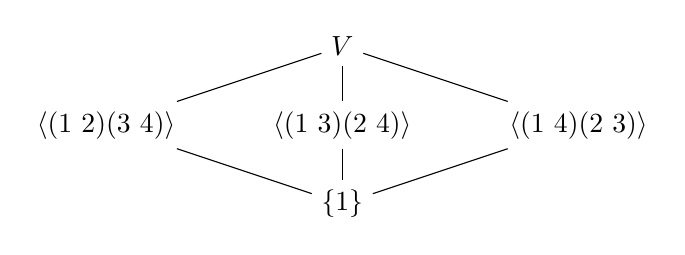
\begin{tikzpicture}[node distance=1cm]
                \node (V) {$V$};
                \node (1) [below of=V, xshift=-3cm] {$\left\langle (1\ 2)(3\ 4)\right\rangle$};
                \node (2) [below of=V] {$\left\langle (1\ 3)(2\ 4)\right\rangle$};
                \node (3) [below of=V, xshift=3cm] {$\left\langle (1\ 4)(2\ 3)\right\rangle$};
                \node (4) [below of=2] {$\{1\}$};

                \draw (V) -- (1);
                \draw (V) -- (2);
                \draw (V) -- (3);
                \draw (1) -- (4);
                \draw (2) -- (4);
                \draw (3) -- (4);
            \end{tikzpicture}    
            \caption{Diagrama de Hasse para los subgrupos del grupo de Klein.}
            \label{fig:ej11_V}
        \end{figure}
        \item El grupo simétrico $S_3$.
        
        Sabemos que $|S_3|=6$. Por el Teorema de Lagrange, sabemos que los subgrupos de $S_3$ han de tener orden 1, 2, 3 o 6. El subgrupo de orden 1 es $\{1\}$, y el subgrupo de orden 6 es $S_3$. Veamos ahora los subgrupos de orden 2 y 3. Como $2$ y $3$ son primos, entonces los subgrupos de orden 2 y 3 han de ser cíclicos. Sabemos que:
        \begin{equation*}
            S_3=\{1,(1\ 2),(1\ 3),(2\ 3),(1\ 2\ 3),(1\ 3\ 2)\}
        \end{equation*}
                
        Por tanto, los subgrupos de orden 2 son:
        \begin{align*}
            \langle (1\ 2)\rangle &= \{1,(1\ 2)\}\\
            \langle (1\ 3)\rangle &= \{1,(1\ 3)\}\\
            \langle (2\ 3)\rangle &= \{1,(2\ 3)\}
        \end{align*}

        Por otro lado, los subgrupos de orden 3 son:
        \begin{align*}
            \langle (1\ 2\ 3)\rangle &= \{1,(1\ 2\ 3),(1\ 3\ 2)\}
        \end{align*}
        Notemos que no ha hecho falta calcular $\langle (1\ 3\ 2)\rangle$ puesto que, $\langle x\rangle=\langle x^{-1}\rangle$. Por tanto, el retículo de subgrupos de $S_3$ es el de la Figura~\ref{fig:ej11_S3}.
        \begin{figure}
            \centering
            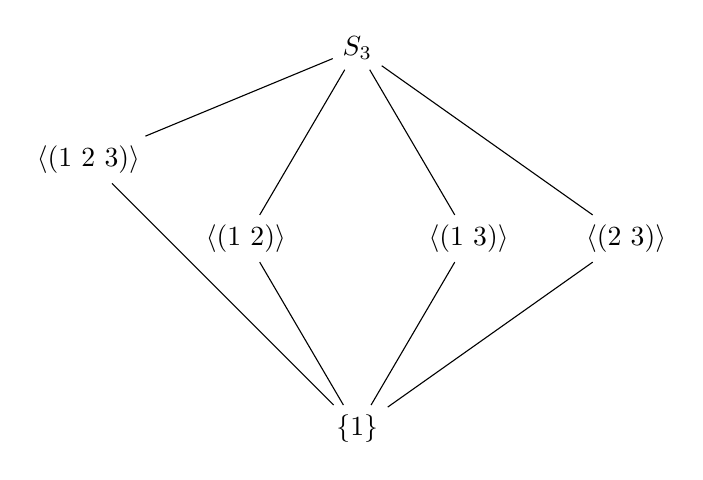
\begin{tikzpicture}[node distance=2cm]
                \node (S3) {$S_3$};
                \node (1) [below left of=S3, yshift=-1cm] {$\left\langle (1\ 2)\right\rangle$};
                \node (2) [below right of=S3, yshift=-1cm] {$\left\langle (1\ 3)\right\rangle$};
                \node (3) [left of=1, yshift=1cm] {$\left\langle (1\ 2\ 3)\right\rangle$};
                \node (4) [right of=2] {$\left\langle (2\ 3)\right\rangle$};
                \node (5) [below right of=1, yshift=-1cm] {$\{1\}$};
                
                \draw (S3) -- (1);
                \draw (S3) -- (2);
                \draw (S3) -- (3);
                \draw (S3) -- (4);
                \draw (1) -- (5);
                \draw (2) -- (5);
                \draw (3) -- (5);
                \draw (4) -- (5);
            \end{tikzpicture}
            \caption{Diagrama de Hasse para los subgrupos de $S_3$.}
            \label{fig:ej11_S3}
        \end{figure}
        \item El grupo diédrico $D_4$.
        
        Sabemos que $|D_4|=8$. Por el Teorema de Lagrange, sabemos que los subgrupos de $D_4$ han de tener orden 1, 2, 4 u 8. El subgrupo de orden 1 es $\{1\}$, y el subgrupo de orden 8 es $D_4$. Veamos ahora los subgrupos de orden 2 y 4. Como $2$ es primo, entonces los subgrupos de orden 2 han de ser cíclicos. Sabemos que:
        \begin{equation*}
            D_4=\{1,r,r^2,r^3,s,sr,sr^2,sr^3\}
        \end{equation*}

        Calculemos el orden de los elementos de $D_4$:
        \begin{gather*}
            O(1) =1\qquad O(r)=O(r^3)=4\\
            O(r^2)=O(s)=O(sr)=O(sr^2)=O(sr^3)=2
        \end{gather*}

        Por tanto, los subgrupos de orden 2 son:
        \begin{align*}
            \langle r^2\rangle &= \{1,r^2\}\\
            \langle s\rangle &= \{1,s\}\\
            \langle sr\rangle &= \{1,sr\}\\
            \langle sr^2\rangle &= \{1,sr^2\}\\
            \langle sr^3\rangle &= \{1,sr^3\}
        \end{align*}

        Calculamos ahora los subgrupos de orden 4. Sabemos que:
        \begin{equation*}
            \langle r\rangle = \{1,r,r^2,r^3\}=\langle r^3\rangle
        \end{equation*}

        No obstante, busquemos más grupos de orden $4$, algo que no será sencillo.
        Dado un subgrupo $H$, como $H=\langle H\rangle$, entonces siempre podemos encontrar un conjunto de generadores suyo. Buscaremos por tanto conjuntos de generadores con $1$, $2$, $3$ y $4$ elementos.
        \begin{itemize}
            \item \ul{Con un elemento:}
            
            Los subgrupos generados por un único elemento sabemos que son cíclicos y el orden del elemento ha de ser el orden del grupo. Por tanto, el único subgrupo de $D_4$ de orden $4$ es:
            \begin{equation*}
                \langle r\rangle = \{1,r,r^2,r^3\} = \langle r^3\rangle
            \end{equation*}

            \item \ul{Con dos elementos:}
            
            A partir de aquí, es más complejo. Sabemos que los generadores no han de ser ni $r$ ni $r^3$, pues estos generarían un grupo de orden mayor que $4$. Además, incluir a $1$ como generador no tiene sentido. Por último, notemos que $x$ y $x^{-1}$ generan el mismo grupo. Las posibles combinaciones son:
            \begin{align*}
                \langle s, r^2\rangle &= \{1,s,r^2,sr^2\}\\
                \langle s, sr\rangle &= D_4\ \text{pues}\ r=s\cdot sr\\
                \langle s, sr^2\rangle &= \langle s, r^2\rangle\ \text{pues}\ s\cdot sr^2=r^2\\
                \langle s, sr^3\rangle &\supset \langle r^3\rangle\ \text{pues}\ s\cdot sr^3=r^3\\
                \langle sr, r^2\rangle &= \{1,sr,sr^3,r^2\}\\
                \langle sr, sr^2\rangle &\supset \langle r\rangle\ \text{pues}\ sr\cdot sr^2=ssr^3r^2=r\\
                \langle sr, sr^3\rangle &= \langle sr,r^2\rangle\ \text{pues}\ sr\cdot sr^3=r^2\\
                \langle r^2, sr^2\rangle &= \langle s, r^2\rangle\ \text{pues}\ sr^2\cdot r^2=s\\
                \langle r^2, sr^3\rangle &= \langle sr, r^2\rangle\ \text{pues}\ sr^3\cdot r^2=sr\\
                \langle sr^2, sr^3\rangle &= D_4\ \text{pues}\ r=sr^2\cdot sr^3\ \text{y}\ sr^3\cdot r=s
            \end{align*}

            Por tanto, y en resumen, los únicos subgrupos de $D_4$ de orden $4$ generados por dos elementos son:
            \begin{align*}
                \langle s, r^2\rangle &= \{1,s,r^2,sr^2\}\\
                \langle sr, r^2\rangle &= \{1,sr,sr^3,r^2\}
            \end{align*}

            \item \ul{Con tres elementos:}
            
            Supongamos (pues en otro caso ya se habría estudiado) que todos los elementos generadores son de orden $2$ y distintos. Sean estos $x$, $y$ y $z$. Como $\langle x,y\rangle$ nos proporciona un subgrupo de orden $4$ o mayor, caben dos posibilidades:
            \begin{itemize}
                \item Al añadir $z$ como generador, no se generen más elementos. En este caso, $\langle x,y,z\rangle=\langle x,y\rangle$, caso ya estudiado.
                \item Al añadir $z$ como generador, se generen más elementos. En este caso, $\langle x,y,z\rangle=D_4$.
            \end{itemize}

            \item \ul{Con cuatro elementos:}
            
            Supongamos (pues en otro caso ya se habría estudiado) que todos los elementos generadores son de orden $2$ y distintos. Entonces, como también el $1$ pertenecerá a dicho subgrupo, tenemos que este grupo será $D_4$.
        \end{itemize}

        Por tanto, los únicos subgrupos de $D_4$ de orden $4$ son:
        \begin{align*}
            \langle r\rangle &= \{1,r,r^2,r^3\} = \langle r^3\rangle\\
            \langle s, r^2\rangle &= \{1,s,r^2,sr^2\}\\
            \langle sr, r^2\rangle &= \{1,sr,sr^3,r^2\}
        \end{align*}

        Por tanto, el retículo de subgrupos de $D_4$ es el de la Figura~\ref{fig:ej11_D4}.
        \begin{figure}
            \centering
            \begin{tikzpicture}[node distance=2cm]
                \node (D4) {$D_4$};
                \node[below of=D4] (r) {$\langle r\rangle$};
                \node[left of=r] (r2s) {$\langle s, r^2\rangle$};
                \node[right of=r] (r2sr) {$\langle sr, r^2\rangle$};
                \node[below of=r] (r2) {$\langle r^2\rangle$};
                \node[left of=r2] (sr2) {$\langle sr^2\rangle$};
                \node[right of=r2] (sr3) {$\langle sr^3\rangle$};
                \node[right of=sr3] (sr) {$\langle sr\rangle$};
                \node[left of=sr2] (s) {$\langle s\rangle$};
                \node[below of=r2] (1) {$\{1\}$};

                \draw (D4) -- (r);
                \draw (D4) -- (r2s);
                \draw (D4) -- (r2sr);
                \draw (r) -- (r2);
                \draw (r2s) -- (sr2);
                \draw (r2s) -- (s);
                \draw (r2s) -- (r2);
                \draw (r2sr) -- (sr3);
                \draw (r2sr) -- (sr);
                \draw (r2sr) -- (r2);
                \draw (r2) -- (1);
                \draw (sr2) -- (1);
                \draw (sr3) -- (1);
                \draw (sr) -- (1);
                \draw (s) -- (1);
            \end{tikzpicture}
            \caption{Diagrama de Hasse para los subgrupos de $D_4$.}
            \label{fig:ej11_D4}
        \end{figure}



        \item El grupo cuaternio $Q_2$.
        
        Sabemos que $|Q_2|=8$. Por el Teorema de Lagrange, sabemos que los subgrupos de $Q_2$ han de tener orden 1, 2, 4 u 8. El subgrupo de orden 1 es $\{1\}$, y el subgrupo de orden 8 es $Q_2$. Veamos en primer lugar el orden de los elementos de $Q_2$:
        \begin{gather*}
            O(1)=1\qquad O(-1)=2\qquad O(\pm i)=O(\pm j)=O(\pm k)=4
        \end{gather*}

        Como $2$ es primo, los subgrupos de orden $2$ han de ser cíclicos y generados por un elemento de orden $2$. Por tanto, el único subgrupo de orden $2$ es:
        \begin{equation*}
            \langle -1\rangle = \{1,-1\}
        \end{equation*}

        Respecto a los subgrupos de orden $4$, buscaremos conjuntos de generadores de $1,2,3$ y $4$ elementos.
        \begin{itemize}
            \item \ul{Con un elemento:}
            
            Los subgrupos generados por un único elemento sabemos que son cíclicos y el orden del elemento ha de ser el orden del grupo. Por tanto, estos son:
            \begin{align*}
                \langle i\rangle &= \{1,i,-1,-i\}\\
                \langle j\rangle &= \{1,j,-1,-j\}\\
                \langle k\rangle &= \{1,k,-1,-k\}
            \end{align*}

            \item \ul{Con dos elementos:}
            
            Supongamos (pues en otro caso ya se habría estudiado) que los generadores no son de orden $4$. Entonces tan solo puede ser el $1$ y el $-1$, caso ya estudiado. Por tanto, no consideramos ni este caso ni los generados por más elementos.
        \end{itemize}

        Por tanto, el retículo de subgrupos de $Q_2$ es el de la Figura~\ref{fig:ej11_Q2}.
        \begin{figure}
            \centering
            \begin{tikzpicture}[node distance=2cm]
                \node (Q2) {$Q_2$};
                \node (1) [below of=Q2, xshift=-2cm] {$\left\langle i\right\rangle$};
                \node (2) [below of=Q2] {$\left\langle j\right\rangle$};
                \node (3) [below of=Q2, xshift=2cm] {$\left\langle k\right\rangle$};
                \node (4) [below of=2] {$\left\langle -1\right\rangle$};
                \node (5) [below of=4] {$\{1\}$};

                \draw (Q2) -- (1);
                \draw (Q2) -- (2);
                \draw (Q2) -- (3);
                \draw (1) -- (4);
                \draw (2) -- (4);
                \draw (3) -- (4);
                \draw (4) -- (5);
            \end{tikzpicture}
            \caption{Diagrama de Hasse para los subgrupos del grupo de los cuaternios.}
            \label{fig:ej11_Q2}
        \end{figure}
        


        \item El grupo alternado $A_4$.
        
        Sabemos que $|A_4|=12$. Por el Teorema de Lagrange, sabemos que los subgrupos de $A_4$ han de tener orden 1, 2, 3, 4, 6 o 12. El subgrupo de orden 1 es $\{1\}$, y el subgrupo de orden 12 es $A_4$. Veamos ahora los subgrupos de orden 2, 3, 4 y 6. Para ello, antes de nada, mostremos los elementos de $A_4$:
        \begin{multline*}
            A_4=\{1,(1\ 2\ 3),(1\ 2\ 4),(1\ 3\ 2),(1\ 3\ 4),(1\ 4\ 2),(1\ 4\ 3),(2\ 3\ 4),(2\ 4\ 3),\\ (1\ 2)(3\ 4),(1\ 3)(2\ 4),(1\ 4)(2\ 3)\}
        \end{multline*}

        Como $V<A_4$, entonces los subgrupos de $V$ son subgrupos de $A_4$. Estos son:
        \begin{align*}
            \langle (1\ 2)(3\ 4)\rangle &= \{1,(1\ 2)(3\ 4)\}\\
            \langle (1\ 3)(2\ 4)\rangle &= \{1,(1\ 3)(2\ 4)\}\\
            \langle (1\ 4)(2\ 3)\rangle &= \{1,(1\ 4)(2\ 3)\}\\
            V&= \langle (1\ 2)(3\ 4),(1\ 3)(2\ 4)\rangle
        \end{align*}

        Veamos si hay más subgrupos de orden $2$. Como $2$ es primo, estos han de ser cíclicos generados por un elemento de orden $2$; pero no hay más elementos de orden $2$ en $A_4$. Por tanto, los subgrupos de orden $2$ son los anteriormente mencionados.\\

        Veamos ahora los subgrupos de orden $3$. Como $3$ es primo, estos han de ser cíclicos generados por un elemento de orden $3$. Además, hemos de tener en cuenta que $\langle x\rangle=\langle x^{-1}\rangle$. Por tanto, los subgrupos de orden $3$ son:
        \begin{align*}
            \langle (1\ 2\ 3)\rangle &= \{1,(1\ 2\ 3),(1\ 3\ 2)\}\\
            \langle (1\ 2\ 4)\rangle &= \{1,(1\ 2\ 4),(1\ 4\ 2)\}\\
            \langle (1\ 3\ 4)\rangle &= \{1,(1\ 3\ 4),(1\ 4\ 3)\}\\
            \langle (2\ 3\ 4)\rangle &= \{1,(2\ 3\ 4),(2\ 4\ 3)\}
        \end{align*}

        Veamos ahora los subgrupos de orden $4$. Como $4$ no es primo, no es tan sencillo. Buscaremos que estén generados por $1$, $2$, $3$ y $4$ elementos.
        \begin{itemize}
            \item \ul{Con un elemento:}
            
            Los subgrupos generados por un único elemento sabemos que son cíclicos y el orden del elemento ha de ser el orden del grupo. Como no hay elementos de orden $4$, no hay subgrupos de orden $4$ generados por un único elemento.

            \item \ul{Con dos elementos:}
            
            Supongamos (pues en otro caso ya se habría estudiado) que los dos elementos son distintos y de orden $2$ (pues el orden de todo elemento debe dividir al orden del subgrupo al que pertenece). Entonces, llegamos al grupo de Klein, caso ya estudiado. Por tanto, no consideramos generadores de más elementos.
        \end{itemize}

        Respecto a los subgrupos de orden $6$, en el ejemplo de la página~\pageref{ejemplo:subgrupos_a4} se vió que no existen subgrupos de orden $6$ en $A_4$. Por tanto, el retículo de subgrupos de $A_4$ es el de la Figura~\ref{fig:ej11_A4}.
        \begin{figure}
            \centering
            \begin{tikzpicture}[node distance=2cm]
                \node (A4) {$A_4$};
                \node (V) [below of=A4, xshift=3.5cm] {$V$};
                \node (1) [below of=V, xshift=-2.5cm, yshift=-2cm] {$\left\langle (1\ 2)(3\ 4)\right\rangle$};
                \node (2) [below of=V, yshift=-2cm] {$\left\langle (1\ 3)(2\ 4)\right\rangle$};
                \node (3) [below of=V, xshift=2.5cm, yshift=-2cm] {$\left\langle (1\ 4)(2\ 3)\right\rangle$};
                \node (4) [below of=A4, xshift=-1.5cm, yshift=-2cm] {$\left\langle (1\ 2\ 3)\right\rangle$};
                \node (5) [left of=4] {$\left\langle (1\ 2\ 4)\right\rangle$};
                \node (6) [left of=5] {$\left\langle (1\ 3\ 4)\right\rangle$};
                \node (7) [left of=6] {$\left\langle (2\ 3\ 4)\right\rangle$};

                \node (8) [below of=A4, yshift=-6.5cm] {$\{1\}$};

                \draw (A4) -- (V);
                \draw (V) -- (1);
                \draw (V) -- (2);
                \draw (V) -- (3);
                \draw (A4) -- (4);
                \draw (A4) -- (5);
                \draw (A4) -- (6);
                \draw (A4) -- (7);
                \draw (1) -- (8);
                \draw (2) -- (8);
                \draw (3) -- (8);
                \draw (4) -- (8);
                \draw (5) -- (8);
                \draw (6) -- (8);
                \draw (7) -- (8);
            \end{tikzpicture}
            \caption{Diagrama de Hasse para los subgrupos del grupo alternado $A_4$.}
            \label{fig:ej11_A4}
        \end{figure}
    \end{enumerate}

\end{ejercicio}

\begin{ejercicio}\label{ej:3.12}
    Fijado un número primo $p$, describe el retículo de subgrupos del grupo cíclico $C_{p^n}$. En particular, describe el retículo de subgrupos del grupo cíclico $C_8$.\\

    Sabemos que, para cada divisor de $p^n$, existe un subgrupo de $C_{p^n}$ de ese orden. En concreto, los únicos subgrupos de $C_{p^n}$ son los de la forma $\langle x^{p^k}\rangle$ con $k\in \{0,\ldots,n\}$. Además:
    \begin{equation*}
        O(x^{p^k})=\dfrac{O(x)}{\mcd(O(x),p^k)}=\dfrac{p^n}{\mcd(p^n,p^k)}=\dfrac{p^n}{p^k}=p^{n-k}
    \end{equation*}

    Por tanto, $\langle x^{p^k}\rangle=C_{p^{n-k}}$. Además, fijado $k\in \{0,\ldots,n\}$, tenemos que $\langle x^{p^{k+1}}\rangle\subset \langle x^{p^{k}}\rangle$, puesto que $x^{p^{k+1}}=(x^{p^k})^{p}$.    
    Por tanto, el retículo de subgrupos de $C_{p^n}$ es el de la Figura~\ref{fig:ej12}.
    \begin{figure}
        \centering
        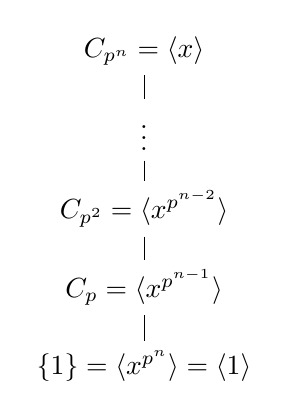
\begin{tikzpicture}[node distance=1cm]
            \node (G)  {$C_{p^n}=\langle x\rangle$};
            \node[below of=G] (p) {$\vdots$};
            \node[below of=p] (p2) {$C_{p^2}= \langle x^{p^{n-2}}\rangle$};
            \node[below of=p2] (p1) {$C_{p}= \langle x^{p^{n-1}}\rangle$};
            \node[below of=p1] (1) {$\{1\}= \langle x^{p^{n}}\rangle= \langle 1\rangle$};

            \draw (G) -- (p);
            \draw (p) -- (p2);
            \draw (p2) -- (p1);
            \draw (p1) -- (1);
        \end{tikzpicture}
        \caption{Retículo de subgrupos de $C_{p^n}$ para el Ejercicio~\ref{ej:3.12}.}
        \label{fig:ej12}
    \end{figure}

    En particular, para $C_8$, tenemos que $p=2$ y $n=3$. Por tanto, el retículo de subgrupos de $C_8$ es el de la Figura~\ref{fig:ej12_8}.
    \begin{figure}
        \centering
        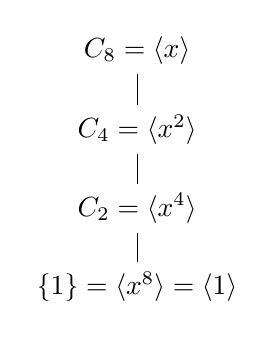
\begin{tikzpicture}[node distance=1cm]
            \node (G)  {$C_8=\langle x\rangle$};
            \node[below of=G] (p2) {$C_{4}= \langle x^{2}\rangle$};
            \node[below of=p2] (p1) {$C_{2}= \langle x^{4}\rangle$};
            \node[below of=p1] (1) {$\{1\}= \langle x^{8}\rangle= \langle 1\rangle$};

            \draw (G) -- (p2);
            \draw (p2) -- (p1);
            \draw (p1) -- (1);
        \end{tikzpicture}
        \caption{Retículo de subgrupos de $C_8$ para el Ejercicio~\ref{ej:3.12}.}
        \label{fig:ej12_8}
    \end{figure}
\end{ejercicio}

\begin{ejercicio}\label{ej:3.13}
    Demostrar que un grupo finito $G \neq \{1\}$ carece de subgrupos propios, esto es, que su retículo de subgrupos es el de la Figura~\ref{fig:ej13} si, y sólo si, $G = C_p$ es un grupo cíclico de orden primo.
    \begin{figure}
        \centering
        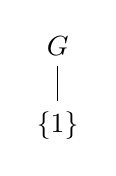
\begin{tikzpicture}[node distance=1cm]
            \node (G)  {$G$};
            \node[below of=G] (1) {$\{1\}$};

            \draw (G) -- (1);
        \end{tikzpicture}
        \caption{Retículo de subgrupos de para el Ejercicio~\ref{ej:3.13}.}
        \label{fig:ej13}
    \end{figure}

    \begin{description}
        \item[$\Longrightarrow)$] Supongamos que $G$ es un grupo finito que carece de subgrupos propios. Como $G\neq \{1\}$, sea $x\in G\setminus \{1\}$. Entonces, $\langle x\rangle\neq \{1\}$ es un subgrupo de $G$; y como este no es propio, entonces $\langle x\rangle=G$. Por tanto, $G$ es cíclico.
        
        Por último, por ser $G$ cíclico sabemos que, por cada divisor de $|G|$, existe un subgrupo de $G$ de ese orden. Como $G$ no tiene subgrupos propios, entonces los únicos divisores de $|G|$ son $1$ y $|G|$. Por tanto, $|G|$ es primo.

        \item[$\Longleftarrow)$] Supongamos que $G=C_p$ es un grupo cíclico de orden primo. Sabemos que, por cada divisor de $|G|$, existe un subgrupo de $G$ de ese orden. Como $|G|=p$ es primo, entonces los únicos divisores de $|G|$ son $1$ y $|G|$. Por tanto, $G$ carece de subgrupos propios.
    \end{description}
\end{ejercicio}

\begin{ejercicio}\label{ej:3.14}
    Describir los retículos de subgrupos de los grupos cíclicos siguentes:
    \begin{enumerate}
        \item $C_6$.
        
        Sabemos que los subgrupos propios de $C_6$ son de la forma $\langle x^k\rangle$ con $k\in \{2,3\}$. Además, $O(x^k)=\frac{6}{\mcd(6,k)}=\frac{6}{k}$. Por tanto, estos son:
        \begin{align*}
            \langle x^2\rangle &= \{1,x^2,x^4\}\\
            \langle x^3\rangle &= \{1,x^3\}
        \end{align*}

        Por tanto, el retículo de subgrupos de $C_6$ es el de la Figura~\ref{fig:ej14_6}.
        \begin{figure}
            \centering
            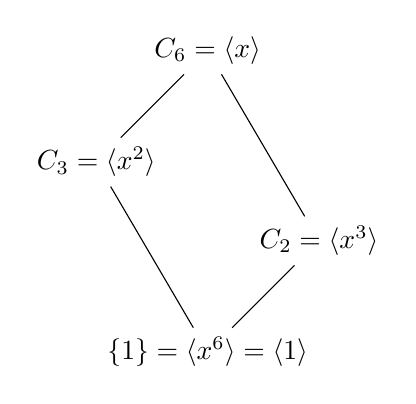
\begin{tikzpicture}[node distance=2cm]
                \node (G)  {$C_6=\langle x\rangle$};
                \node[below left of=G] (p2) {$C_{3}= \langle x^{2}\rangle$};
                \node[below right of=G, yshift=-1cm] (p1) {$C_{2}= \langle x^{3}\rangle$};
                \node[below left of=p1] (1) {$\{1\}= \langle x^{6}\rangle= \langle 1\rangle$};
    
                \draw (G) -- (p2);
                \draw (G) -- (p1);
                \draw (p2) -- (1);
                \draw (p1) -- (1);
            \end{tikzpicture}
            \caption{Retículo de subgrupos de $C_6$ para el Ejercicio~\ref{ej:3.14}.}
            \label{fig:ej14_6}
        \end{figure}
        \item $C_{12}$.
        
        Sabemos que los subgrupos propios de $C_{12}$ son de la forma $\langle x^k\rangle$ con $k\in \{2,3,4,6\}$. Además, $O(x^k)=\frac{12}{\mcd(12,k)}=\frac{12}{k}$. Por tanto, estos son:
        \begin{align*}
            \langle x^2\rangle &= \{1,x^2,x^4,x^6,x^8,x^{10}\}\\
            \langle x^3\rangle &= \{1,x^3,x^6,x^9\}\\
            \langle x^4\rangle &= \{1,x^4,x^8\}\\
            \langle x^6\rangle &= \{1,x^6\}
        \end{align*}

        Por tanto, el retículo de subgrupos de $C_{12}$ es el de la Figura~\ref{fig:ej14_12}.
        \begin{figure}
            \centering
            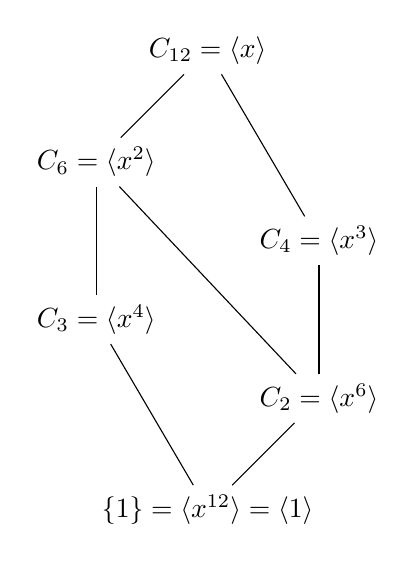
\begin{tikzpicture}[node distance=2cm]
                \node (G)  {$C_{12}=\langle x\rangle$};
                \node[below left of=G] (p2) {$C_{6}= \langle x^{2}\rangle$};
                \node[below right of=G, yshift=-1cm] (p1) {$C_{4}= \langle x^{3}\rangle$};
                \node[below of=p2] (p3) {$C_{3}= \langle x^{4}\rangle$};
                \node[below of=p1] (p4) {$C_{2}= \langle x^{6}\rangle$};
                \node[below left of=p4] (1) {$\{1\}= \langle x^{12}\rangle= \langle 1\rangle$};
    
                \draw (G) -- (p2);
                \draw (G) -- (p1);
                \draw (p2) -- (p3);
                \draw (p1) -- (p4);
                \draw (p4) -- (p2);
                \draw (p3) -- (1);
                \draw (p4) -- (1);
            \end{tikzpicture}
            \caption{Retículo de subgrupos de $C_{12}$ para el Ejercicio~\ref{ej:3.14}.}
            \label{fig:ej14_12}
        \end{figure}
    \end{enumerate}
\end{ejercicio}

\begin{ejercicio}\label{ej:3.15}
    Se considera el grupo cíclico $C_{136}$ de orden 136, con generador $t$. ¿Qué relación hay entre los subgrupos $H_1 = \langle t^{48}, t^{72} \rangle$ y $H_2 = \langle t^{46} \rangle$?\\

    Estudiamos en primer lugar el grupo $H_2$. Como $O(t)=136$, entonces:
    \begin{equation*}
        H_2 = \langle t^{46}\rangle = \langle t^{\mcd(136,46)}\rangle = \langle t^2\rangle
    \end{equation*}

    Por otro lado:
    \begin{align*}
        H_1 &= \langle t^{48}, t^{72}\rangle = \langle t^{48}\rangle \vee \langle t^{72}\rangle = \langle t^{\mcd(136,48)}\rangle \vee \langle t^{\mcd(136,72)}\rangle\\
        &= \langle t^8\rangle \vee \langle t^{8}\rangle = \langle t^8\rangle
    \end{align*}

    Por tanto, se nos pide estudiar la relación entre los subgrupos $\langle t^2\rangle$ y $\langle t^8\rangle$. Puesto que $t_8\in \langle t^2\rangle$, entonces:
    \begin{equation*}
        H_1 = \langle t^8\rangle < \langle t^2\rangle = H_2
    \end{equation*}
\end{ejercicio}

\begin{ejercicio}\label{ej:3.16}
    Demostrar que el grupo de unidades $\bb{Z}_7^\times$ es un grupo cíclico.\\

    \begin{description}
        \item[Opción 1.] Veamos que $O(5)=6$:
        \begin{align*}
            5^2 &= 4\\
            5^3 &= 6\\
            5^4 &= 2\\
            5^5 &= 3\\
            5^6 &= 1
        \end{align*}
    
        Por tanto, $\bb{Z}_7^\times = \langle 5\rangle$ es un grupo cíclico.
        
        \item[Opción 2.] Sabemos que $|\bb{Z}_7^\times|=6$. Por el Ejercicio~\ref{ej:3.10}, sabemos que hay dos posibilidades, o bien $\bb{Z}_7^\times$ es cíclico, o bien $\bb{Z}_7^\times\cong D_3$. No obstante, no puede ser isomorfo a $D_3$, puesto que $D_3$ no es abeliano y $\bb{Z}_7^\times$ sí lo es. Por tanto, $\bb{Z}_7^\times$ es cíclico.
    \end{description}
\end{ejercicio}

\begin{ejercicio}\label{ej:3.17}
    Sea $G$ un grupo y sea $C_n$ el grupo cíclico de orden $n$ generado por $x$. Demostrar que:
    \begin{enumerate}
        \item Si $\theta : C_n \to G$ es un homomorfismo de grupos, entonces:
        \begin{equation*}
            O(\theta(x))\mid n, \quad \text{y} \quad \theta(x^k) = \theta(x)^k \quad \forall k \in \{0, \ldots, n - 1\}.
        \end{equation*}

        Para la primera parte, queremos ver que $(\theta(x))^n=1$. Sabemos que:
        \begin{equation*}
            1 = \theta(1) = \theta(x^n) = \theta(x)^n\Longrightarrow
            O(\theta(x))\mid n
        \end{equation*}

        Para ver el segundo resultado, es suficiente ver que, por ser un homomorfismo, de hecho se tiene para todo $k\in \bb{Z}$. 

        \item Para cada $g \in G$ tal que $O(g) \mid n$, existe un único homomorfismo de grupos $\theta_g : C_n \to G$ tal que $\theta_g(x) = g$.
        
        Veamos que $g^n=1$. Como $O(g)\mid n$, existe $m\in \bb{Z}$ tal que $n=m\cdot O(g)$. Por tanto:
        \begin{equation*}
            g^n = g^{m\cdot O(g)} = (g^{O(g)})^m = 1^m = 1
        \end{equation*}

        Por tanto, por el Teorema de Dyck, existe un único homomorfismo de grupos $\theta_g : C_n \to G$ tal que $\theta_g(x) = g$.
        
        \item Si $g \in G$ es tal que $O(g) \mid n$, entonces el morfismo $\theta_g$ es monomorfismo si, y sólo si, $O(g) = n$.\\
        
        Partimos de:
        \begin{equation*}
            \theta_g\ \text{es monomorfismo} \iff \ker(\theta_g) = \{1\}
        \end{equation*}

        Calculemos el núcleo de $\theta_g$:
        \begin{align*}
            \ker(\theta_g) &= \{x\in C_n\mid \theta_g(x)=1\}
            = \{x^k\mid k\in \{0,\ldots,n-1\},\quad \theta_g(x^k)=1\}\\
            &= \{x^k\mid k\in \{0,\ldots,n-1\},\quad g^k=1\}
        \end{align*}

        Como $O(x)=n$, sabemos que $x^k\neq 1$ para $k\in \{1,\ldots,n-1\}$. Por tanto:
        \begin{equation*}
            \ker(\theta_g) = \{1\}\iff g^k\neq 1\ \forall k\in \{1,\ldots,n-1\}\iff O(g)\geq n
        \end{equation*}

        Como partimos de que $O(g)\mid n$, entonces:
        \begin{equation*}
            \theta_g\ \text{es monomorfismo} \iff O(g)=n
        \end{equation*}

        \begin{comment}

        \begin{description}
            \item[$\Longrightarrow)$] Supongamos que $\theta_g$ es monomorfismo, y veamos que $O(g)=n$. Como $O(g)\mid n$, entonces $O(g)\leq n$. Supongamos ahora $m\in \bb{Z}$ tal que $g^m=1$. Entonces:
            \begin{equation*}
                \theta_g(1)=1 =g^m=\theta_g(x)^m=\theta_g(x^m)
            \end{equation*}

            Por ser $\theta_g$ monomorfismo, entonces $x^m=1$, y por tanto $m\geq n$. Por tanto, $O(g)=n$.


            \item[$\Longleftarrow)$] Supongamos que $O(g)=n$, y veamos que $\theta_g$ es monomorfismo. Para ello, calculemos el núcleo de $\theta_g$:
            \begin{align*}
                \ker(\theta_g) &= \{x\in C_n\mid \theta_g(x)=1\}
                = \{x^k\mid k\in \{0,\ldots,n-1\},\quad \theta_g(x^k)=1\}\\
                &= \{x^k\mid k\in \{0,\ldots,n-1\},\quad g^k=1\}
            \end{align*}
            Como $O(g)=n$, entonces $g^k=1\iff k=0$. Por tanto, $\ker(\theta_g)=\{1\}$, y por tanto $\theta_g$ es monomorfismo.
        \end{description}
        \end{comment}
        
        \item Existe un isomorfismo de grupos
        \begin{equation*}
            \cc{U}(\bb{Z}_n) \cong \Aut(C_n),
        \end{equation*}
        dado por $r \mapsto f_r$ para cada $r = 1, \ldots, n-1$ con $\mcd(r, n) = 1$, donde el automorfismo $f_r$ se define mediante $f_r(x) = x^r$.

        En particular, $\Aut(C_n)$ es un grupo abeliano de orden $\varphi(n)$.\\

        Para cada $r\in \{1,\ldots,n-1\}$ con $\mcd(r,n)=1$ (es decir, $r\in \cc{U}(\bb{Z}_n)$), definimos el siguiente automorfismo de $C_n$:
        \Func{f_r}{C_n}{C_n}{x}{x^r}

        Comprobemos en primer lugar que se trata de un automorfismo. Puesto que $C_n\cong \bb{Z}_n$, entonces $C_n$ es abeliano y, de ahí, se tiene de forma directa que $f_r$ es un homomorfismo. Veamos que es inyectivo:
        \begin{itemize}
            \item \ul{Inyectividad:} Supongamos $k,l\in \{0,\ldots,n-1\}$ tales que $f_r(x^k)=f_r(x^l)$. Entonces, $x^{rk}=x^{rl}\Longrightarrow x^{r(k-l)}=1$. Como $O(x)=n$, se tiene que  $n\mid r(k-l)$. Como además $\mcd(r,n)=1$, entonces $n\mid k-l$, tenemos que $k,l\in \{0,\ldots,n-1\}$, entonces $k-l=0$. Por tanto, $k=l$.
        \end{itemize}
        Por tanto, por ser inyectivo y ser $C_r$ finito, entonces $f_r$ biyectivo. Por tanto, $f_r$ es un automorfismo. Esto nos permite definir la siguiente función:
        \Func{\Phi}{\cc{U}(\bb{Z}_n)}{\Aut(C_n)}{r}{f_r}

        Dividimos la demostración en varios aspectos:
        \begin{description}
            \item[Bien definida:] Veamos en primer lugar que $\Phi$ está bien definida. Para ello, consideramos $r,s\in \bb{Z}$ tales que $[r]=[s]$. Entonces, $s=r+tn$ para algún $t\in \bb{Z}$. Veamos que $f_r=f_s$. Supongamos $\langle x\rangle=C_n$. Entonces, para cada $k\in \{0,\ldots,n-1\}$, se tiene que:
            \begin{align*}
                f_r(x^k) &= x^{rk}\\
                f_s(x^k) &= x^{sk}=\left(x^{r+tn}\right)^k=x^{rk}x^{tnk}=x^{rk}\cdot (x^n)^{tk}=x^{rk}\cdot 1=x^{rk}
            \end{align*}

            Por tanto, $f_r=f_s$, y por tanto $\Phi$ está bien definida.

            \item[Homomorfismo:] Veamos ahora que $\Phi$ es un homomorfismo. Para ello, consideramos $r,s\in \cc{U}(\bb{Z}_n)$:
            \begin{equation*}
                \Phi(rs)=f_{rs}\qquad \Phi(r)\circ \Phi(s)=f_r\circ f_s
            \end{equation*}

            Comprobamos que se trata del mismo automorfismo:
            \begin{equation*}
                f_{rs}(x)=x^{rs}=(x^s)^r=f_r(f_s(x))=(f_r\circ f_s)(x)\qquad \forall x\in C_n
            \end{equation*}

            Por tanto, $\Phi$ es un homomorfismo.

            \item[Inyectividad:] Veamos ahora que $\ker(\Phi)=\{1\}$. Para ello, supongamos que $\exists k\in \cc{U}(\bb{Z}_n)\setminus \{1\}$ tal que $\Phi(k)=f_k=id$. Entonces, para $x\in C_n$ con $O(x)=n$, se tiene que:
            \begin{equation*}
                f_k(x)=x^k=x\Longrightarrow x^{k-1}=1\Longrightarrow n\mid k-1
            \end{equation*}

            Como además $k\in \cc{U}(\bb{Z}_n)$, entonces $k<n$, luego $k-1=0$ y por tanto $k=1$. Por tanto, $\ker(\Phi)=\{1\}$, y por tanto $\Phi$ es monomorfismo.

            \item[Sobreyectividad:] Veamos ahora que $\Phi$ es sobreyectivo. Para ello, consideramos $f\in \Aut(C_n)$. Consideramos $x\in C_n$ tal que $\mcd(x,n)=1$, de forma que $C_n=\langle x\rangle$. Entonces, $f(x)\in C_n$, por lo que $f(x)=x^r$ para algún $r\in \{0,\ldots,n-1\}$. Además, como $f$ es un epimorfismo, entonces $C_n=\langle f(x)\rangle=\langle x^r\rangle$. Por tanto, $\mcd(r,n)=1$, y por tanto $r\in \cc{U}(\bb{Z}_n)$. Veamos que $f=f_r$:
            \begin{equation*}
                f(x^k)=f(x)^k=(x^r)^k=x^{rk}=f_r(x^k)\qquad \forall k\in \{0,\ldots,n-1\}
            \end{equation*}

            Por tanto, $\Phi$ es sobreyectivo. Por tanto, $\Phi$ es un isomorfismo.
        \end{description}

        Una vez demostrado eso, como $\cc{U}(\bb{Z}_n)$ es finito, entonces $\Aut(C_n)$ es finito, con:
        \begin{equation*}
            |\Aut(C_n)|=|\cc{U}(\bb{Z}_n)|=\varphi(n)
        \end{equation*}

        Además, como $\cc{U}(\bb{Z}_n)$ es abeliano, entonces $\Aut(C_n)$ es abeliano.
    \end{enumerate}
\end{ejercicio}

\begin{ejercicio}\label{ej:3.18}~
    \begin{enumerate}
        \item Describir explícitamente el grupo de automorfismos $\Aut(C_8)$.
        
        Por el Ejercicio~\ref{ej:3.17}, sabemos que $\Aut(C_8)\cong \cc{U}(\bb{Z}_8)$. Calculemos $\cc{U}(\bb{Z}_8)$:
        \begin{align*}
            \cc{U}(\bb{Z}_8) &= \{1,3,5,7\}
        \end{align*}

        Por tanto, hay cuatro automorfismos en $\Aut(C_8)$, que son $f_1=id$, $f_3$, $f_5$ y $f_7$ (tal y como definíamos en el Ejercicio~\ref{ej:3.17}). Veámoslo explícitamente en la siguiente tabla:
        \begin{table}[H]
            \centering
            \begin{tabular}{c|c|c|c|c}
                $x$ & $f_1(x)$ & $f_3(x)$ & $f_5(x)$ & $f_7(x)$\\
                \hline
                1 & 1 & 1 & 1 & 1\\
                $x$ & $x$ & $x^3$ & $x^5$ & $x^7$\\
                $x^2$ & $x^2$ & $x^6$ & $x^2$ & $x^6$\\
                $x^3$ & $x^3$ & $x$ & $x^7$ & $x^5$\\
                $x^4$ & $x^4$ & $x^4$ & $x^4$ & $x^4$\\
                $x^5$ & $x^5$ & $x^7$ & $x$ & $x^3$\\
                $x^6$ & $x^6$ & $x^2$ & $x^6$ & $x^2$\\
                $x^7$ & $x^7$ & $x^5$ & $x^3$ & $x$
            \end{tabular}
        \end{table}
        
        \item Demostrar que $\Aut(C_8)$ es isomorfo al grupo de Klein.
        
        Por el apartado anterior, sabemos que $|\Aut(C_8)|=4$. Por el Ejercicio~\ref{ej:3.10}, sabemos que hay dos posibilidades, o bien $\Aut(C_8)$ es cíclico, o bien $\Aut(C_8)\cong V$.\\

        Supongamos que $\Aut(C_8)$ es cíclico. Entonces, $\exists f\in \Aut(C_8)\mid O(f)=4$. Para cada $x\in C_8$, tenemos que:
        \begin{align*}
            (f_3\circ f_3)(x)&=f_3(x^3)=x^9=x\\
            (f_5\circ f_5)(x)&=f_5(x^5)=x^{25}=x\\
            (f_7\circ f_7)(x)&=f_7(x^7)=x^{49}=x
        \end{align*}

        Por tanto, $O(f_3)=O(f_5)=O(f_7)=2$, lo cual es una contradicción. Por tanto, $\Aut(C_8)$ no es cíclico, y por tanto $\Aut(C_8)\cong V$.
    \end{enumerate}
\end{ejercicio}